\documentclass[11pt]{article}
\usepackage{icmlko}
\begin{document}

\title{빠진 한 줄이 만든 상관 --- 원핫의 값은 절편도 상호작용도 아니다}
\author{월드모델 실험실}
\date{노트 401 · 2026년 8월 1일}
\maketitle

\begin{abstract}
노트 400이 원핫의 값을 어디서도 설명하지 못한 채 남겼다 --- 드롭아웃이
아이돌(유보 51행)에서 $-0.1039$ 를 앗아가는데 팝업(65행)은 $+0.0276$ 을
번다. 구조가 후보 하나를 지웠다: \textbf{도메인별 점수는 도메인 안
Spearman 이므로 절편은 순위를 못 바꾼다.} 그러면 원핫이 파는 것은
\textbf{상호작용}이어야 한다 --- 나무가 도메인마다 축을 다르게 쓰게 해 주는
것. 사전 등록했다: \emph{축$\to$라벨 지도가 판 평균에서 많이 어긋난 도메인일
수록 드롭아웃에 많이 잃는다.}

첫 번째 셈이 $\rho = -0.564$ 를 냈다. 사전 등록한 방향이고 곁가지 후보(축
관측률 $+0.067$)를 압도했다. \textbf{채택하지 않았다}(노트 133). 갈라 보니
그 수치는 \textbf{내가 만든 것}이었다.

\begin{center}
\begin{tabular}{lrr}
\hline
드롭아웃 손해와의 순위상관 & 팝업 빼고 & \textbf{전부} \\
\hline
어긋남(날것) & $-0.564$ & $-0.291$ \\
학습 행 수 & $+0.685$ & $+0.264$ \\
\textbf{초과배}(어긋남 $\div$ 잡음 바닥) & --- & $\mathbf{+0.018}$ \\
\hline
\end{tabular}
\end{center}

집계에서 팝업이 \textbf{조용히 빠져 있었다} --- 쓸 축이 셋 미만이라
문턱에 걸렸는데, 하필 \textbf{이야기를 깨는 바로 그 도메인}이었다. 넣고
다시 재고, 어긋남을 그 도메인 크기에서 나오는 \textbf{잡음 바닥}으로 나누자
상호작용 가설은 $\rho = +0.018$ 로 \textbf{완전히 죽었다}. 세 후보(크기,
상호작용, 축 결측)가 모두 죽었고 원핫의 값은 \textbf{미지}로 남는다.
\end{abstract}

\section{잡음 바닥}

작은 도메인의 축$\to$라벨 $\rho$ 는 그냥 흔들린다. 도메인이 판 지도를 정확히
따르더라도 관측 $n$ 행에서 잰 $|\rho_d - \rho_{\text{판}}|$ 의 기대값은
$\sqrt{2/\pi}\,/\sqrt{n-3}$ 근처다. 아이돌은 학습 122행이라 바닥이 $0.080$
인데 잰 어긋남이 $0.139$, 웹툰은 2{,}941행이라 바닥 $0.015$ 에 어긋남
$0.031$ --- \textbf{둘 다 바닥의 두 배쯤}이다. 날것으로 비교하면 작은
도메인이 자동으로 ``어긋난'' 도메인이 된다. 그래서 어긋남과 학습 행 수의
상관이 $-0.427$ 로 나온다. \textbf{어긋남은 크기의 그림자였다.}

바닥으로 나눈 초과배로 다시 세우면 순위가 흩어진다 --- 애니 $3.78$,
세계애니 $3.48$, 펀딩 $3.46$ 이 위쪽인데 이 셋은 드롭아웃에 거의 안 잃거나
(세계애니는) 오히려 번다. 아이돌은 $1.73$ 으로 중간인데 제일 크게 잃는다.

\section{팝업은 잴 수 없다}

팝업의 학습 행은 \textbf{24행}이다. 잰 어긋남 $0.179$ 에 잡음 바닥
$0.221$ --- \textbf{바닥이 더 높다}. 팝업의 축 지도는 판 평균과 같지도
다르지도 않고 \textbf{측정 불가}다. 노트 378 ④의 정신이 여기에도 적용된다:
\emph{잴 수 없는 것은 미결정이 아니라 잴 수 없음이다.}

그런데 팝업은 원핫 실험의 \textbf{유일한 반례}다 --- 24행짜리 도메인이
드롭아웃에 12/12 로 번다. 이 한 줄을 문턱이 조용히 걷어내자 남은 열 도메인은
깔끔한 이야기를 만들었다. \textbf{반례를 지우면 무엇이든 상관이 된다.}

\section{남은 것}

\begin{tabular}{lp{7.4cm}}
\hline
원핫의 값 & \textbf{관측으로 둔다.} 크기·상호작용·축 결측이 다 죽었다.
확정된 것은 절편이 아니라는 구조적 사실 하나뿐 \\
집계 문턱 & 도메인을 거르는 문턱은 전부 \textbf{누가 빠졌는지 찍고} 지나가야
한다 --- 이번엔 반례가 빠졌다 \\
세 번째 전이 짝 & CN 만화 2025+ 19행 --- 더 모으거나 다른 도메인 \\
\hline
\end{tabular}

\begin{figure}[h]
\centering
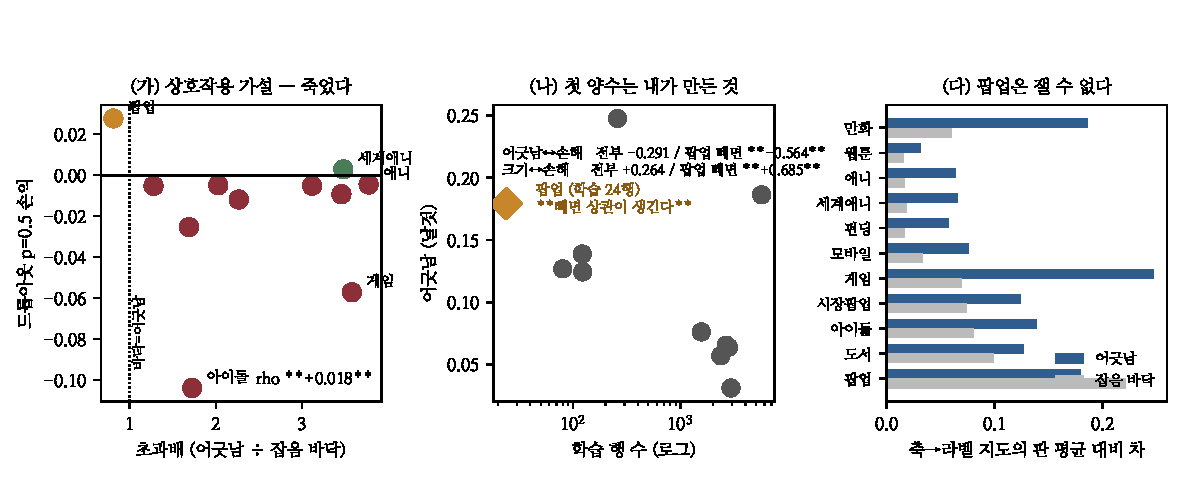
\includegraphics[width=\textwidth]{figs/fig401.pdf}
\caption{(가) 잡음 바닥으로 나눈 초과배는 드롭아웃 손해와 아무 관계가 없다
($\rho = +0.018$). (나) 팝업(마름모, 학습 24행)을 빼면 어긋남↔손해가
$-0.291 \to -0.564$ 로, 크기↔손해가 $+0.264 \to +0.685$ 로 커진다 --- 두
상관 다 이 한 점이 만든다. (다) 팝업만 잡음 바닥이 어긋남보다 높다 ---
잴 수 없다.}
\end{figure}

\end{document}
